\documentclass{subfiles}
\begin{document}
\section{Quantum Mechanics}
\subsection{The Schrödinger equation}
The physical description of any quantum system, i.e the \emph{state space}, is given by the quantum mechanical \emph{wavefunction} (also often called a \emph{state vector})\cite{nielsen2010quantum}, which in Dirac notation is written as $\ket{\Psi(t)}$. 
This function is a complex-valued function that gives a complete description of both static and dynamic properties of a given quantum system, and thus presents the analogue to the classical notion of a set of trajectories in phase space \cite{hochstuhl2014time}. 

The dynamics of the wavefunction is governed by the \emph{Time-dependent Schrödinger Equation} (TDSE),
\begin{equation}
    i\frac{\partial}{\partial t}\ket{\Psi(x, t)} = H(x,t)\ket{\Psi(x, t)}\label{eq:tdse}
\end{equation}
where $H$ a linear hermitian operator often referred to as the \emph{Hamiltonian} \cite{griffiths2018introduction, berera2021quantum}. Here $x$ is the position of the particle, and $t$ is the time. 
This operator describes the total energy of the system, and is given by (in atomic units)
\begin{align*}
    H = -\nabla^2 + V(x)
\end{align*}
where $\nabla^2$ is the Laplacian operator, and $V(x)$ is the potential energy of the system, both external and internal.
This equation gives the equation of motion for the wavefunction, and describes how the wavefunction evolves in time. Atomic units (a.u) transform fundamental constants like the speed of light $c$, Planck's constant $\hbar$, and the electron mass $m_e$ to unity, to simplify equations and calculations. This is a common practice in quantum mechanics, as it allows for easier manipulation of the equations without loss of generality. In this notation, lengths are measured in Bohr radii ($ a_0 = 0.529Å$), energies in Hartees ($ \text{Ha} = 27.211 eV$) and time in  \cite{szabo1996modern}.


While the TDSE govern the time-evolution of the quantum system, many problems - particularly stationary or bound-state problems - are often more easily analysed through the \emph{Time-independent Schrödinger Equation} (TISE), which is obtained by separating the temporal and spatial variables in the TDSE. This gives us
\begin{equation}
    H\ket{\psi_n(x)} = E_n\ket{\psi_n(x)}\label{eq:tise},
\end{equation}
where $\psi_n(x)$ are the \emph{energy eigenstates} of the system, and $E_n$ are the corresponding \emph{energy eigenvalues}. As is clear from the equation \eqref{eq:tise}, the energy eigenvalues are the diagonal elements of the diagonalized Hamiltonian operator. In practice, these eigenvalues are obtained by diagonalizing the Hamiltonian operator (regardless of time-dependency), and the associated eigenvectors forming a basis of energy eigenfunctions. \\

The energy eigenstates are the stationary states of the system, and they form a complete orthonormal basis for the Hilbert space of the system. This means that any wavefunction can be expressed as a linear combination of the energy eigenstates, and in our work, it will serve as an important reference point to validate our choice basis sets. To be precise, any state function $\Psi(x, t)$ can be expressed as a linear combination of the energy eigenstates $\psi_n(x)$ as
\begin{align*}
    \Psi(x, t) = \sum_n c_n\psi_n(x)
\end{align*}
where $c_n$ are the coefficients of the linear combination, which are determined by the initial conditions of the system. This is a direct consequence of the linearity of the Schrödinger equation, and it allows us to express any state function as a superposition of energy eigenstates \cite{griffiths2018introduction, berera2021quantum}.

%% 2nd quantization
\subsection{Second Quantization}
As the earliest formulations of quantum mechanics introduced the ground-breaking concept that physical properties such as energy, momentum and angular momentum are inherently quantized, this formulation is now often referred to as "first quantization". In first quantization, observables are represented by linear operators with real eigenvalues and each individual particle is assigned a wavefunction in a fixed $N$-dimensional Hilbert space.
However, as the theory matured, it became clear that first quantization was inadequate to describe true many-body systems - like systems with indistinguishable particles, where one must (anti-)symmetrize the $N-$ particle wavefunction, or natural processes like particle creation and annihilation, as occurs in chemical reactions or in high-energy physical processes. In these cases the wavefunction must account for all possible particle configurations (outcomes), which quickly becomes unwieldy. The number of terms grows exponentially with the number of particles, making both manipulation and storage intractable \cite{helgaker2013molecular, szabo1996modern}\\

Second quantization solves this problem by introducing a new mathematical framework, which accounts for both the particle indistinguishability and the creation and annihilation of particles, and makes the statefunction also expressed in terms of operators. Furthermore, second quantization allows for a more intuitive and compact notation for many-body systems, where instead of asking "where is particle $i$?", we ask "how many particles are in \emph{state} $i$?". \cite{szabo1996modern, shavitt2009many, helgaker2013molecular}. As such, second quantization is often referred to as the "occupation number representation" of quantum mechanics. This moves the focus from the individual particles to the orbitals they occupy. This reformulation also reduces much of the manipulation of the wavefunction to algebraic operations, which makes numerical implementations more efficient, and easier to understand \cite{helgaker2013molecular}.
\\ 

In second quantization, we introduce a set of creation and annihilation operators, $a^\dagger$ and $a$, which create and annihilate particles in a given state. An important thing to note, is that these operators differ depending on the type of particles. For bosons, these operators satisfy the following commutation relations:
\begin{align}
    [a_i, a_j] = [a^\dagger_i, a^\dagger_j] = 0, \quad [a_i, a^\dagger_j] = \delta_{ij}\label{eq:commutation}
\end{align}
where $[A, B] = AB - BA$, and for fermions, the \emph{anti-}commutation relations are:
\begin{align}
    \{a_i, a_j\} = \{a^\dagger_i, a^\dagger_j\} = 0, \quad \{a_i, a^\dagger_j\} = \delta_{ij}\label{eq:anti_commutation}
\end{align}
where $\{A, B\} = AB + BA$.
\textcolor{red}{TODO: Nice section but is it necessary to include? Yeah we probably need to, as we have the section on Fock space (which we need. Should probably make sure to mention fock space more explicitly further on?)}
%% FOCKSPACE
\subsection{Fock Space}\textcolor{red}{TODO: We are not really using the Fock space, that is not where our product states live. Should we maybe exclude this section? What to replace it with? We kinda use the Fock Space when we compare anti-symmetric states to our distinguishable product states, but we do not use the Fock space formalism. Maybe we should just mention it briefly, and then refer to the literature?}
In the framework of second quantization, the concept of a \emph{Fock space}\footnote{First introduced by V. A. Fock in \cite{fock1932konfigurationsraum}} emerge naturally as a mathematical structure for describing quantum systems with variable, or uknown, number of particles. A Fock space is a direct sum of Hilbert spaces, 
\begin{align*}
    \mathcal{F} = \bigotimes_{n=0}^\infty S_{\pm} \mathcal{H}_n
\end{align*}
where each space, $\mathcal{H}_n$ represents a state with fixed a number of particles, and $S_{\pm}$ is the symmetrization operator for bosons ($+$) and fermions ($-$). Meaning, the zero-particle states, one-particle states, two-particle states etc. This encapsulates all possible configurations of a many-body system elegantly. Using the occupation number representation introduced in second quantization, a state in Fock space is not expressed by momenta or position, but rather by the number of particles occupying certain quantum states\cite{helgaker2013molecular}. 
\\

For instance, the state $\ket{n_1, n_2, ...}$ informs that $n_1$ particles occupy state $1$, $n_2$ particles  in state $2$. The annihilation and creation operators act on the Fock states by increasing, or decreasing, the occupation numbers of the corresponding states. Meaning, the action of the creation operator on a state is given by
\begin{align*}
    a^\dagger_i\ket{n_1, n_2, ...} = \sqrt{n_i + 1}\ket{n_1, n_2, ..., n_i + 1, ...}.
\end{align*}
and the action of the hermitian conjugate annihilation operator is given by
\begin{align*}
    a_i\ket{n_1, n_2, ...} = \sqrt{n_i}\ket{n_1, n_2, ...,n_i-1, n_i - 1, ...}.
\end{align*}
From this, these operators can describe particle interactions, transitions and dynamics in a many-body system. As the Fock space is constructed by direct sums, two states of different particle numbers are inherently orthogonal, i.e. $\braket{n|m} = \delta_{nm}$, where $n$ and $m$ are the number of particles in the two states. This orthogonality is crucial for the mathematical consistency of the notation \cite{helgaker2013molecular, shavitt2009many}.
\\

For systems of indistinguishable particles, Fock spaces naturally incorporate the Pauli exclusion principle, as the anti-commutation relations \eqref{eq:anti_commutation} ensure that no two fermions can occupy the same quantum state. This fundamental property of fermions explains, for example, why electrons in an atom cannot share identical quantum numbers. For bosonic systems (distinguishable particles), the commutation relations \eqref{eq:commutation} instead allow multiple particles to occupy the same state, which is crucial for phenomena such as Bose-Einstein condensation \cite{pethick2008bose}.


\subsection{Hartree approximation}\label{sec:hartree_theory}
Accurately solving the Schrödinger equation for many-body systems is a formidable challenge—even a one-dimensional system with just a few interacting particles can become intractable very quickly. The core difficulty stems from the exponential growth of the Hilbert space as we add more degrees of freedom, coupled with particle interactions and, for identical particles, the need to enforce antisymmetry (the Pauli exclusion principle). In real-world applications—like molecular dynamics or solid-state physics - we often invoke the Born-Oppenheimer\footnote{Formulated by Max Born and Robert J. Oppenheimer in their 1927 paper \cite{Born_Oppenheimer_1927}} approximation to freeze out the nuclear motion, which drastically reduces the size of the electronic Hilbert space \cite{helgaker2013molecular, szabo1996modern}. Even after that simplification, however, finding an exact solution on a classical computer remains out of reach.
\\ 

Mean-field methods offer a practical way to approximate the many-body problem by replacing the full interacting Hamiltonian with an effective single-particle picture in which each particle feels an average field created by all the other particles. In quantum chemistry, the most familiar mean-field approach is Hartree-Fock (HF), which assumes the wavefunction is a single Slater determinant of orthonormal orbitals. A detailed derivation of the Hartree-Fock procedure can be found in appendix \ref{app:HF_theory}. Those orbitals are determined self-consistently, meaning iteratively until convergence, so that each one “sees” the averaged Coulomb repulsion (direct term) and exchange interactions from all the other electrons. \textcolor{red}{TODO: Maybe re-write this part to clarify clearly that we are using Hartree instead of HF? Kinda wierd transition into the variational principle.}
\\
Central to any mean-field approach is the variational principle, which asserts that the expectation value of the energy
\begin{equation}
    E[\Psi] = \frac{\braket{\Psi|H|\Psi}}{\braket{\Psi|\Psi}}\label{eq:variational_principle},
\end{equation}
is always greater than or equal to the true ground state energy $E[\Psi]\geq E_0$. By choosing a trial wavefunction $\Psi$ with adjustable parameters (here, the single-particle orbitals), we can minimize this expectation value until it converges to a local minimum\cite{helgaker2013molecular}\footnote{We refer the reader particularly to chapter 4.2 in \cite{helgaker2013molecular}}. 

In Hartee-Fock theory this trial wavefunction is a slater-determinant; in Hartree, it becomes a simple product of single-particle orbitals, often called a \emph{Hartree product}. These single-particle orbitals are the solution of the one-electron Schrödinger equation, 
\begin{align*}
    \hat{h}\phi_i = \epsilon_i\phi_i
\end{align*}
where the full Hamiltonian (for a non-interacting) system would be 
\begin{align*}
    H = \sum_{i=1}^N \hat{h}_i
\end{align*}
which has the solution eigenvector
\begin{align}
    \Psi = \phi_1(\mathbf{r}_1)\phi_2(\mathbf{r}_2)...\phi_N(\mathbf{r}_N)\label{eq:hartree_product}
\end{align}
with corresponding eigenvalue $E = \epsilon_1 + \epsilon_2 + ... + \epsilon_N$, i.e. the sum of single-particle energies. Equation \eqref{eq:hartree_product} is the Hartree product, and it is the simplest possible wavefunction for a many-body system. As is evident, this Hartree product is not anti-symmetric, nor indistinguishable, as the particles are designated a specific orbital to occupy and thus they are distinguishable, and the state is symmetric under particle exchange.

\\
In our double-well system, the two particles remain localized in separate wells and therefore behave like distinguishable subsystems rather than identical fermions. We still employ a mean-field strategy—now in the form of a Hartree approach—where the full two-particle wavefunction is approximated as a simple product of two single-particle orbitals (one in each well). Each orbital is chosen so that it minimizes the energy in the presence of the averaged Coulomb field generated by the other particle. This “bipartite Hartree” procedure allows us to incorporate the essential interaction effects while keeping the computational effort manageable.

\\
To derive this method, we select a finite basis set $\{\chi_\alpha\}$ for each subsystem $M$ (left or right well), and expand the single-particle Hartree orbitals in this basis. 
\begin{align*}
    \ket{\phi^M_i} = \sum_{\alpha=1}^{N^M} C^M_{\alpha i}\ket{\chi_\alpha}
\end{align*}
where $N^M$ is the number of single-particle basis functions in subsystem $M$. The Hartree product state for our two-particle system can then be expressed as a product of the single-particle Hartree orbitals for each subsystem, i.e. $\ket{\phi^A_i}$ and $\ket{\phi^B_j}$, where $i,j$ are the orbital indices for subsystems A and B respectively. We can then also define the two necessary integrals, the one-body integrals and the two-body interaction integrals, as
\begin{align*}
    h_{\alpha\beta}^M &= \bra{\chi_\alpha^M}h^M\ket{\chi_\beta^M} = \int \chi_\alpha^{M*} h^M\chi_\beta^M d\mathbf{r},\\
    u_{\alpha\beta,\gamma\delta} &= \bra{\chi_\alpha^M\chi_\beta^N}u^{MN}\ket{\chi_\gamma^M\chi_\delta^N}, = \int \chi_\alpha^{M*}\chi_\beta^{N*} u^{MN} \chi_\gamma^M\chi_\delta^N d\mathbf{r}_M d\mathbf{r}_N
\end{align*}
where $h^M$ is the single-body Hamiltonian for subsystem $M$, and $u^{MN}$ is the two-body interaction between subsystems $M$ and $N$. The two-body interaction is the Coulomb interaction between the two subsystems. Due to the nature of our system, where the particls occupy distinct wells, we can omit the otherwise present exchange term in the two-body interaction integral and only the direct coulomb interaction remains. \\


The groundstate wavefunction will then have the following form:
\begin{align*}
    \ket{\Psi} = \ket{\phi^A_0\phi^B_0}
\end{align*}
where $\phi_0^M$ is the single-particle Hartree functions (orbitals) for subsystem $M\in[A,B]$, with the constraint that these single-particle orbitals are orthonormal. We can set up the Lagrangian
\begin{align*}
    L = E_H - \lambda^A(\braket{\phi^A_0|\phi^A_0} - 1) - \lambda^B(\braket{\phi^B_0|\phi^B_0} - 1)
\end{align*}
where $\lambda^M$ are the Lagrange multipliers, and $E_H$ is the Hartree energy, which is the expectation value of the Hamiltonian in the Hartree product state
\begin{align*}
    E_H = \bra{\Psi}H\ket{\Psi} = \bra{\phi^A_0}h^A\ket{\phi^A_0} + \bra{\phi^B_0}h^B\ket{\phi^B_0} + \braket{\phi^A_0\phi^B_0|u^{AB}|\phi^A_0\phi^B_0}
\end{align*}
here $h^M$ are the single-body Hamiltonian, for each subsystem and $u^{AB}$ the mean-field Coulomb interaction between subsystems. The Hartree orbitals can be expanded in our single-particle basis set, as linear combinations, 
\begin{align*}
    \ket{\phi^M_i} = \sum_{\alpha=1}^{N^M} C^M_{\alpha i}\ket{\chi_\alpha}
\end{align*}
where $N^M$ is the number of single-particle basis functions in subsystem $M$. Minimizing the Lagrangian by the basis transformation cofficients $C_{\alpha 0}^M$ gives us two coupled eigenvalue equations, i.e calculating $\partial L/\partial C_{\alpha 0}^{M*} = 0$ for $M\in[A,B]$ yields
\begin{align}
    &\frac{\partial L}{\partial C_{\alpha 0}^{A*}}  = \sum_{\beta=0}^{N_A}\big(h_{\alpha\beta}^A + \sum^{N_B}_{\gamma\delta=0}C^{B*}_{\gamma0} u_{\alpha\gamma,\beta\delta}C^B_{\delta0} \big)C^A_{\beta 0}  = \lambda^AC^A_{\alpha 0},\nonumber \\
    &\frac{\partial L}{\partial C_{\alpha 0}^{B*}}  = \sum_{\beta=0}^{N_B}\big(h_{\alpha\beta}^B + \sum^{N_A}_{\delta\gamma=0}C^{A*}_{\delta0} u_{\delta\alpha,\gamma\beta}C^A_{\gamma0} \big)C^B_{\beta 0}  = \lambda^BC^B_{\alpha 0}.\label{eq:bipartite_hartree}
\end{align}
where $\h_{\alpha\beta} = \bra{\chi_\alpha^M}h^M\ket{\chi_\beta^M}$ are the one-body integrals, and $u_{\alpha\beta,\gamma\delta} = \bra{\chi_\alpha^M\chi_\beta^N}u^{MN}\ket{\chi_\gamma^M\chi_\delta^N}$ are the two-body interaction integrals.  \\\\
These eigenvalue equations are for subsystem A and B respectivly, and we can identify the \emph{Hartree matrix} (similar to the Fock matrix in Hartree-Fock theory, omitting the exchange term) as the LHS inside the big paranthesis. These two coupled equations are solved iteratively, by updating the coefficients $C_{\alpha 0}^M$ until convergence is reached (self-consistency). By diagonalization of these Hartree matrices we gain the $N_M$ lowest energy orbitals $C^M_{\alpha i}$ and energy levels $\lambda^M_i=\epsilon^M_i$\cite{leinonen2024coulomb}, which we will use as our single-particle basis for each subsystem. The equations to be solved are
\begin{align}
    \sum_{\beta=0}^{N_M} f_{\alpha\beta}^M C^M_{\beta i} = \epsilon_i^M C^M_{\alpha i}\label{eq:hartree_eigenvalue}
\end{align}
with the Hartree matrices from eqs. \ref{eq:bipartite_hartree}. From this we identify the \emph{Hartree operator}
\begin{equation}
    f_{\alpha\beta}^M \;=\; h_{\alpha\beta}^M
    \;+\;\sum_{\gamma,\delta=0}^{N_{\bar M}}
      C_{\gamma0}^{\bar M\,*}\;u_{\alpha\gamma,\beta\delta}\;C_{\delta0}^{\bar M}.
\label{eq:hartree_operator}
\end{equation}

This method to solve the interacting many-body problem is called the Hartree method, and is a simplification of the Hartree-Fock method where Hartree product states are applied, instead of anti-symmtric Slater determinants. This method will natually introduce a mean-field coulomb interaction between our two subsystems into their respective basis sets, and will be the basis for our study of the two-particle syste \cite{leinonen2024coulomb}.
%%% CONFIGURATION INTERACTION
\subsection{Configuration Interaction}\label{sec:CI}
Configuration Interaction (CI) refines the mean-field Hartree solution by expanding on the Hartree product state to include all possible configurations of the particles. The exact two-body wavefunction is then expanded in a basis of \emph{correlated} product states, which are constructed from the single-particle Hartree orbitals. This allows us to account for all possible correlations between the particles, and thus obtain a more accurate description of the system. If we include all possible configurations (i.e infinite number of basis states) we obtain Full Configuation Interaction (FCI), which is the exact solution to the many-body problem, but is intractable for all but the smallest systems \cite{helgaker2013molecular, szabo1996modern}. \\

Starting from the Hartree orbitals for subsystem A and B (obtained by solving the eigenvalue equations \ref{eq:hartree_eigenvalue}), we can collect a truncated set of single-particle orbitals, $\{\phi^A_i\}$ and $\{\phi^B_j\}$, where $i,j<N$ are the orbital indices for subsystems A and B respectively, and $M=N^2$ is the number of single-particle orbitals we include in our basis set, and construct all possible two-particle product states
\begin{align*}
    \phi_i^A(\mathbf{r}_1)\phi_j^B(\mathbf{r}_2).
\end{align*}  
As mentioned, retaining all such product states leads to the exact solution within the one-particle basis approximation, but due to the combinatorial explosion of the number of product states, we choose to truncate the basis set include $N$ function in each subsystem. 

To enforce the Pauli exclusion principle - and regaining exhange effects omitted by the distinguishable-particle Hartree product - we construct anti-symmetrized linear combinations of the Hartree product states. Each such unorordered pair $(i,j)$ gives a Slater-type state
\begin{align*}
    \ket{\Psi_{ij}} = \frac{1}{\sqrt{2}}(\phi_i^A(\mathbf{r}_1)\phi_j^B(\mathbf{r}_2) - \phi_j^A(\mathbf{r}_1)\phi_i^B(\mathbf{r}_2)).
\end{align*}
which is equivalent to the Slater determinant\footnote{We refer the reader to ch. 2.2.3 in \cite{szabo1996modern} for details on the Slater Determinant}\textcolor{red}{TODO: Should we include theory on the SD?} for two particles in two different subsystems, that is, when accounting for the strict localization of the two particles the particle-swap terms are zero in the determinant. 

Gathering all unique such pairs $i<j$ of Slater-type states, yields a basis set of $N^2$ two-particle states. We then build the many-body Hamiltonian matrix in this basis set, which is given by
\begin{align*}
    H_{ij,kl} = \bra{\Psi_{ij}}H\ket{\Psi_{kl}} = \bra{\phi_i^A\phi_j^B}H\ket{\phi_k^A\phi_l^B}
\end{align*}
by evaluating the one- and two-body integrals in the truncated CI basis, and diagonalizing it to obtain the CI eigenvalues and eigenvectors. 

The energy difference
\begin{align*}
    \Delta E = E^{\text{Hartree}} - E^{\text{CI}}
\end{align*}
quantifies the correlation energy captured by the CI method within our truncated orbital space. This correlation energy is a measure of how well our distinguishable treatment of our system approximates the true many-body wavefunction, and is a key indicator for the validity of our approach.\textcolor{red}{TODO: Add more on how CI can be used to validate our two-qubit gate protocol further.}


%%% MORSE  POTENTIAL
\subsection{Morse potential}\label{sec:morse_potential}
To build our qubit system, we need to define some form of potential trap that we can confine our particles within. In modern quantum computing many different potentials are used, tested and theorized. One of the most common potentials are the Quantum Harmonic Oscillator potential (QHO), a very well known potential in quantum mechanics. This potential has been studied in great detail and has been used in many different quantum systems, and is very often used as a benchmark for more advanced symmetric potentials \cite{griffiths2018introduction, berera2021quantum}. The QHO basis sets are widely employed to study quantum dot systems\cite{Yuan_2017}, and are often used in quantum chemistry to describe molecular vibrations \cite{atkins2011molecular}. 
\\ 

One could think that using the QHO potential for our qubit would be a natural choice, but there are some nuances necessary to consider. The QHO double well potential is perfectly symmetric, meaning the energy levels are uniformly spaced, and equal across both wells. This is not ideal for qubit systems, as we need more control over eneregy levels in both wells - and the uniform energy spacing makes one-qubit operations unstable as we lack control over what energy levels we excite \cite{devoret2013superconducting}. 

To achieve this, we will instead use the Morsee potential, first introduced by Philip M. Morse in 1929 as a solution to the Schrödinger equation representing the motion of the nuclei in a diatomic molecule\cite{morse1929diatomic}. This potential has non-uniform energy levels, and more parameters, and is widely used in quantum mechanics to describe anharmonic oscillators. An extension of the Morse potential, Morse/Long-rangee potential is one of the most popular potentials to model potential energy surfaces used for spectroscopy\cite{zhai2018constructing}. Given that this potential has already seen alot of study within quantum dot systems, and molecular systems in general, it is natural to belive that this potential, should we succeed in our study, prove to be a promising candidate for a prototype (near) room-temperature qubit system\cite{khordad2014linear, hayrapetyan2015exciton, sargsian2021effects}. \\

The Morse potential is given as
\begin{align*}
    V(r) = De^{-2a(r-r_0)} - 2De^{-a(r-r_0)}
\end{align*}
This function has a minima of $-D$ at $r = r_0$, and goes asymptotically towards zero at $r=\infty$, and tends towards large values for $r\rightarrow0$. In our study, we will rewrite the potential somewhat, to make it more computationally efficient to make multiple evaluations. As the zero-point of a potential is arbitrary, we can subtract or add any scalar valuee without loss of generality. We will therefore rewrite the Morse potential, adding the zero-point energy $D$ to the potential, and factor out a $D$ to simplify the expression. This gives us
\begin{align*}
    V(r) &= De^{-2a(r-r_0)} - 2De^{-a(r-r_0)} + D \\
    &= D(e^{-2a(r-r_0)} - 2e^{-a(r-r_0)} + 1)
\end{align*}
which yields a simpler form, by factorization using the square binomial formula,
\begin{align}
    V = D(e^{-a(r-r_0)} - 1)^2\label{eq:morse_potential}
\end{align}
where now, computationally, we need only evaluate the exponential function once, and the rest of the potential is simple algebraic operations. This makes our computations more efficient, as the evaluation of the expoenntial function is computationally expensive, since computing exponentials generally requires many more CPU cycles than simple arithmetic, it is advantageous to reduce their number. Here the $D$ parameter is the dissociation energy, which is the depth of the potential well, and $a$ is a parameter that controls the width of the well, and thus the curvature of the potential. The parameter $r_0$ is the position of the well minima, and can be used to shift the potential to any desired position.\\

Expanding a Taylor series about the well minima, we can see that the potential is approximatively harmonic. From this, we can identify Hookes law, and also identify the spring constant in this potential. Expanding around $r_0$
\begin{align*}
    V(r) = V(r_0) + V'(r_0)(r-r_0) + \frac{1}{2}V''(r_0)(r-r_0)^2 + ...
\end{align*}
and, since we are operating around the minima, higher order terms can be neglected as they become very small ($\Delta r^n = (r - r_0)^n\to 0$ for $n>2$\textcolor{red}{TODO: Should we instead writ this as $\mathcal{O}(\Delta r^n)$? or something along these lines.}). By shifting the zero point of the potential to $r_0$, we have $V(r_0) = 0$. Furthermore, as $r_0$ is a minima of the potential, $V'(r_0) = 0$, as the slope of the potential function is flat at this point\textcolor{red}{TODO: This is a trivial statement, do we need to cite or prove?}. This simplifies our expression to
\begin{align*}
    V(r) = \frac{1}{2}V''(r_0)(r-r_0)^2
\end{align*}
which we identify as the harmonic oscillator potential, with the spring constant $k = V''(r_0)$, and if we, by differentiation w.r.t $r$, use it to find the force on a particle we indentify Hooke's Law. This gives us a new parameter to control the width of the well, and the curvature of the potential, which is expressed as
\begin{align*}
    V' &= 2D(1 - e^{-a(r-r_0)})a \\
    V'' &= 2Da^2e^{-a(r-r_0)} \\
    V''(r_0) &= 2Da^2 \\
    k &= 2Da^2 \rightarrow a = \sqrt{\frac{k}{2D}}
\end{align*} 
\begin{figure}[h!]
    \centering
    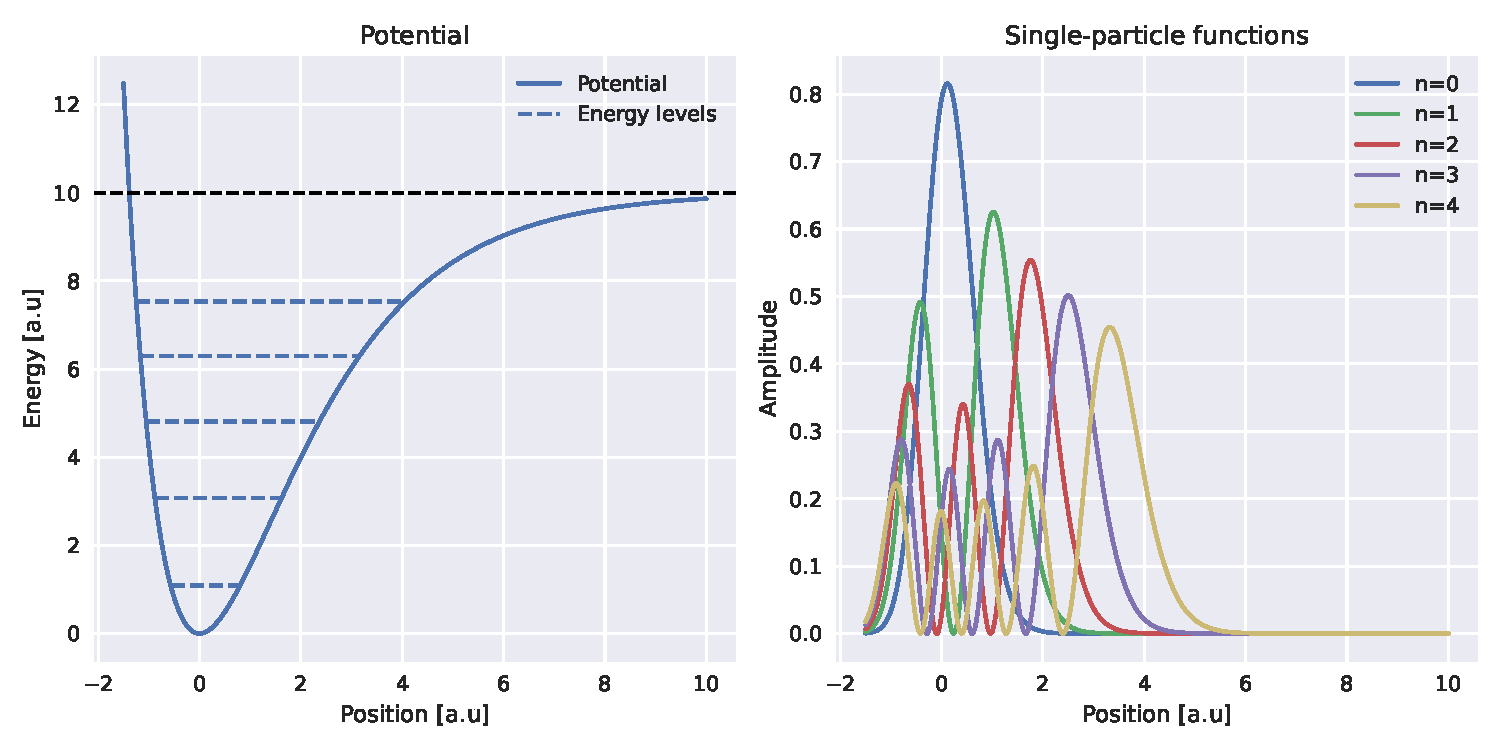
\includegraphics[width=1.0\textwidth]{figs/potential_spf.pdf}
    \caption{The Morse potential and the 5 lowest energy levels and energy eigenfunctions. Dissociation energy, $D$, is highlighted by the black dashed line, and the parameters for this visualization of a Morse potential are $D=10, a=0.5, x_0=0$. We can see how the lowest lying states are populatied near the well minima, while the higher order states are spreading out further towards the dissacociation curve (to the right), as opposed to the potential wall at the left side. The energy levels are anharmonic, and the spacing non-uniform, as is expected from the Morse potential. }
    \label{fig:morse_potential}
\end{figure}
Figure \ref{fig:morse_potential} shows the Morse potential, with the 5 lowest energy levels and corresponding energy eigenfunctions. \\


%% Double well
Now, we would like to make a potential trap for \emph{two} separate particles, as our qubit system will be a two-particle system. To do so, we construct a double Morse potential well, simply by adding two Morse potentials together. We flip the right potential well, so that the minima are at the same position, and the potential is symmetric (given symmetric parameters). This gives us the double Morse potential as
\begin{equation}
    V(r) = D_L(e^{-a_L(r-r_{0,L})} - 1)^2 + D_R(e^{a_R(r-r_{0,R})} - 1)^2\label{eq:double_well_morse_potential}
\end{equation}
where the subscripts L and R correspond to left and right well, respectively. The parameter $D$ controls the depth of the potential well, whilst $a$ has some control over the width of the well, through the steepness of the exponential functions decay (and thus the curvature, and width, of the well). A smaller $a$ parameter constitues a wider well as the function would then decay slowly, recall also this parameters relation with the spring-like constant $k=2Da^2$, which is the parameter we shall use instead\textcolor{red}{TODO: Change the expressions for the potentials so that $k$ is used instead? Or leave as is?}. The parameter $r_0$ is the position of the well minima. It is this potential that we shall study in great detail in this thesis, and we will use it to construct our qubit system. The parameters will be tuned throughout the time-evolution to achieve the desired energy level structure, and thus control the qubit system parametrically.

\begin{figure}[h!]
    \centering
    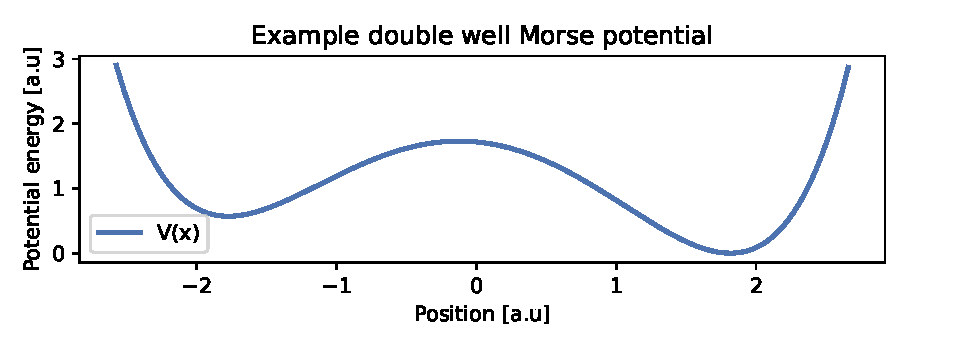
\includegraphics[width=1.0\textwidth]{figs/double_well_potential.pdf}
    \caption{A visual representation of the double Morse potential, with the two wells, and the energy levels. Parameters for this visualization are $D_L=10$, $D_R=11$, $k_l=7$, $k_r=7$, $r_{0,L}=-2$, $r_{0,R}=2$, with a grid length of $5.3$, with $N=400$ grid points. The deviance between well depths ($D_L \neq D_R$) is what gives the asymmetrical shape of the potential, and subsequently will give degenerate single-particle energy levels.} 
    \label{fig:double_well_morse_potential}
\end{figure}
Figure \ref{fig:double_well_morse_potential} shows the double Morse potential, with the two wells. This is an example visualization, and shows how the qubit system can be constructed by tuning the parameters of the potential and placing a single particle in each well minima. With a sufficiently high barrier between the two wells, we can ensure that the particles remain localized in their respective wells, and thus behave like distinguishable subsystems. The asymmetric shape of the potential is due to the difference in well depths, $D_L \neq D_R$, which will give us distinct single-particle energies in each well, and thus a non-degenerate energy level structure.  
\end{document}